\section{Punti di estensione} \label{section:punti_estensione}

ShopChain è un'applicazione progettata pensando anche ad eventuali operazioni future di manutenzione o
estensione del prodotto: durante lo sviluppo dell'applicazione ShopChain sono stati esplorati vari spunti per nuove features e ampliamenti, 
che però a causa del poco tempo rimasto non sono state implementate in tempo.
Sono state individuate principalmente tre aree che potranno essere ampliate.

\subsection{TheGraph protocol}

Nella pagina di visualizzazione degli ordini il gruppo ha implementato la possibilità di filtrare gli ordini restituiti direttamente dalla blockchain. Attualmente questa funzionalità è fornita solo tramite un controllo a front-end, in futuro si potrebbe evolvere la funzione di filtraggio tramite l'implementazione del protocollo TheGraph\glo{}.

The Graph è un protocollo decentralizzato per indicizzare e successivamente effettuare query dei dati presenti in blockchain in una modalità simile a quella che avviene con una normale base di dati. Questo permette di interrogare la blockchain in modo facile e veloce, ed estraendo dati che altrimenti non sarebbe possibile visualizzare.

In particolare quanto citato è possibile tramite la creazione di subgraph. Un sottografo non è altro che una serie di parametri necessari al protocollo per poter mappare e creare un indice dei dati presenti in blockchain.\\
Si compongono di tre componenti principali:

\begin{itemize}
 \item Manifest (subgraph.yaml) che definisce quali dati il sottografo andrà a indicizzare;

 \begin{figure}[H]
    \centering
    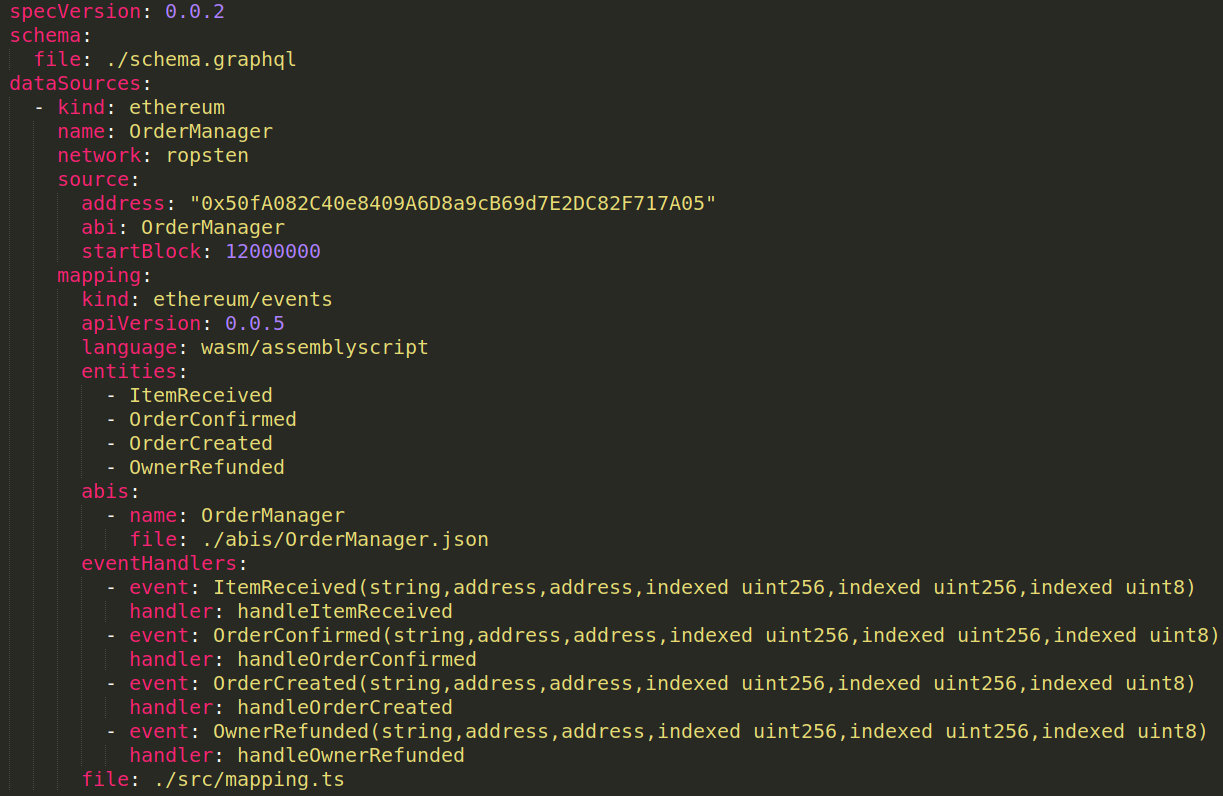
\includegraphics[scale=0.3]{immagini/subgraf.png}
    \caption{Esempio di un possibile subgraph configurato per il contratto OrderManager per la rete Ropsten.}
 \end{figure}


 \item Schema (schema.graphql) che riporta quali dati si desidera ricevere dal sottografo;

 \begin{figure}[H]
    \centering
    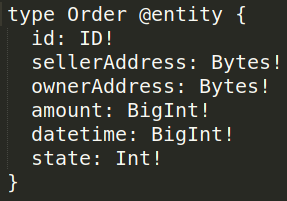
\includegraphics[scale=0.4]{immagini/schema.png}
    \caption{Esempio di file schema per la definizione entità Order.}
 \end{figure}

 \item AssemblyScript Mappings (mapping.ts) file che riporta la traduzione dei dati presenti in blockchain che il sottografo dovrà indicizzare.

 \begin{figure}[H]
    \centering
    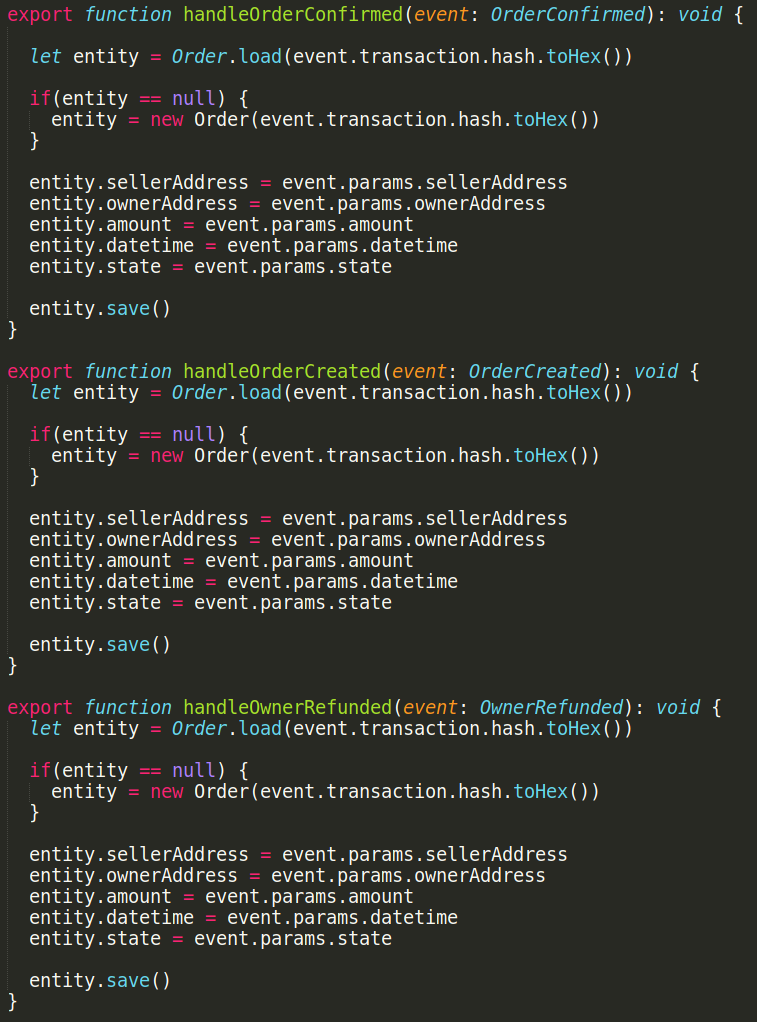
\includegraphics[scale=0.3]{immagini/map.png}
    \caption{Esempio di file mapping per l'indicizzazione degli eventi.}
 \end{figure}

\end{itemize}

Questa funzionalità non è stata portata avanti perché non è disponibile sulla testnet di Fantom, ma solo sulla mainnet. Se la si vuole implementare sarà quindi necessario eseguire lo sviluppo e i relativi test su una testnet di Ethereum in cui è disponibile il protocollo (es. Rinkeby\glo). Una volta che lo sviluppo sarà finito si potrà procedere a caricare il subgraph creato sulla mainnet di Fantom senza particolari modifiche, poiché quest'ultima è una blockchain EVM.


\subsection{Chain differenti}

Un ovvio ampliamento per l'applicazione è il supporto a più blockchain, per raggiungere un bacino di utenza più ampio e garantire quindi un maggior successo dell'applicazione.\\


\subsection{Frontend}

\subsubsection{Immagine MoneyBox}

Il gruppo aveva pensato di associare ad ogni MoneyBox una immagine generata automaticamente, o presa da un pool di immagini definito. Se si sceglie di generarla automaticamente, si può prendere come seed di generazione uno tra i seguenti: l'id dell'ordine associato alla MoneyBox, 
il numero del blocco relativo alla transazione in blockchain, il timestamp della creazione.
Questo contribuisce ad una maggiore sicurezza nel condividere il link alla suddetta MoneyBox con amici, che potranno vedere a colpo d'occhio se il link è corretto tramite l'immagine incorporata.

\subsubsection{Riflettere i cambiamenti del contratto}

Con i cambiamenti che possono venire apportati agli smart contract è bene che il lato frontend dell'applicazione sia aggiornato di conseguenza.
Nel caso dei cambiamenti proposti finora i cambiamenti individuati sono i seguenti:
\begin{itemize}
    \item \textbf{TheGraph}: le due pagine di elenco transazioni dovranno essere modificate per sfruttare appieno tutte le funzionalità portate dalla implementazione dei protocolli TheGraph;
    \item \textbf{Chain differenti}:  in un pop-up all'ingresso dell'applicazione, l'utente potrà selezionare la chain (e quindi la cryptovaluta correlata) con la quale procedere al pagamento. Tale scelta dovrà essere riportata anche nella breadcrumb come reminder testuale.
\end{itemize}

